%% using aastex version 6
%Write that Einv == Eobs for equation 8 to be true. %[conversation with Steve]
%

\newcommand{\opsfp}{N$_{\rm FP_{\rm obs}}$}
\newcommand{\opspc}{N$_{\rm PC_{\rm obs}}$}
\newcommand{\opsN}{N$_{\rm obs}$}
\newcommand{\trueopspc}{T$_{\rm PC_{\rm obs}}$}
\newcommand{\missedfp}{T$_{\rm FP_{\rm obs}}$ - N$_{\rm FP_{\rm obs}}$}
\newcommand{\invfp}{N$_{\rm FP_{\rm inv}}$}
\newcommand{\invpc}{N$_{\rm PC_{\rm inv}}$}
\newcommand{\invN}{N$_{\rm inv}$}
\newcommand{\sfatce}{sfaTCE}


We use the \injtce, \scrtce, and \invtce\ data sets to determine the performance of the Robovetter and to measure the completeness and the reliability of the catalog. As a reminder, the reliability we are attempting to measure is only the reliability of the catalog against false alarms and does not address the astrophysical reliability (see \S\ref{s:occurates}. As discussed in \S\ref{s:tces}, the long-period \opstces\ are dominated by false alarms and so this measurement is crucial to understand the reliability of some of the most interesting candidates in our catalog.

{\color{blue}
Robovetter completeness, $C$, is the fraction of injected transits detected by the \Kepler\ Pipeline that are passed by the Robovetter as PCs.  As long as the \injtce{s} are representative of the observed PCs, completeness tells us what fraction of the true planets are missing from the final catalog.  Completeness is calculated by dividing the number of on-target \injtce{s} that are dispositioned as PCs (N$_{\rm PC_{\rm inj}}$) by the total number of \injtce{s} (N$_{\rm inj}$).

\begin{equation}
C \approx \frac{N_{\rm PC_{\rm inj}}}{N_{\rm inj}}
\label{e:comp}
\end{equation}

\noindent If the parameter space under consideration becomes too large and there are gradients in the actual completeness, differences between the \injtce and the \opstce{} populations will prevent the completeness measured with Equation~\ref{e:comp} from matching the actual Robovetter completeness. For example, there are more long-period \injtce{s} than short-period ones, which is not representative of the \opstce{s}, the true fraction of candidates correctly dispositioned by the Robovetter is not accurately represented by binning over all periods. With this caveat in mind, we use $C$ in this paper to indicate the value we can measure, as shown in Equation~\ref{e:comp}.

%If the parameter space under consideration does not contain a significant number of injections to be adequately sampled, the measured completeness may not be a good measure of the actual Robovetter completeness. For example, there are a lot more long-period \injtce{s} than short-period ones, there are not many injections at short periods, and thus that region of parameter space may not be well-measured enough, which may be a concern since most \opstces\ are at short periods. With this caveat in mind, we use $C$ in this paper to indicate the value we can measure, as shown in Equation~\ref{e:comp}.
}

The candidate catalog reliability, $R$, is defined as the ratio of the number of PCs which are truly exoplanets (\trueopspc) to the total number of PCs (\opspc) from the \opstce{} data set. 
\begin{equation}
\label{eq:rel}
R = \frac{T_{\rm PC_{\rm obs}}}{N_{\rm PC_{\rm obs}}}
\end{equation}

Calculating the reliability for a portion of the candidate catalog is not straight forward because we do not know which PCs are the true transiting exoplanets and cannot directly determine $T_{\rm PC_{\rm obs}}$. Instead, we use the simulated false alarm data sets to understand how often false alarms sneak past the Robovetter and contaminate our final catalog.


\subsection{Reliability Derivation}
\label{s:relcalc}
To assess the catalog reliability against false alarms, we will assume that the \scrtce{s} and \invtce{s} are similar (in frequency and type) to the \opstces.  One way to calculate the reliability of the catalog from our false alarm sets is to first calculate how often the Robovetter correctly identifies known false alarms as FPs, a value we call effectiveness ($E$).  Then, given the number of FPs we identify in the \opstce\ set, we can determine the reliability of the catalog against the type of false alarms present in the simulated sets (\invtces\ and \scrtces). This method assumes the relative frequency of the different types of false alarms is well emulated by the simulated data sets, but the total number of false alarms need not be well emulated.


Robovetter effectiveness ($E$) is defined as the fraction of FPs correctly identified as false positives in the \opstce\ data set,

\begin{equation}
\label{effect1}
E \equiv \frac{N_{\rm FP_{\rm obs}}}{T_{\rm FP_{\rm obs}}}
\end{equation}

\noindent where $T_{\rm FP_{\rm obs}}$ is the number of FPs which are truly false positives and $N_{\rm FP_{\rm obs}}$ is the total number of measured FPs. Notice we are using $N$ to indicate the measured number, and T to indicate the ``True'' number. 

If the simulated false alarm TCEs accurately reflect the \opstce\ false alarms, $E$ can be estimated as the number of simulated false alarm TCEs identified as FPs (\invfp) divided by the number of inverted TCEs (\invN), 
%assuming $E$~$\leq$~1.
\begin{equation}
\label{effect2}
E \approx E_{\rm inv} \equiv \frac{N_{\rm FP_{\rm inv}}}{N_{\rm inv}}
\end{equation}


For ease of notation we are using inversion to represent the false alarm TCEs, but the same calculation applies when using the combination of both inversion and scrambling, as we do later in the paper. 

{\color{blue}
Recall that the Robovetter makes a binary decision, and TCEs are either PCs or FPs. For this derivation we do not take into consideration the reason the Robovetter calls a TCE an FP (i.e., some false alarms fail because the Robovetter indicates there is a stellar eclipse or centroid offset). For most of parameter space, an overwhelming fraction of FPs are false alarms in the \opstce{} data set. Future studies will look into separating out the effectiveness for different types of FPs using the set of injected astrophysical FPs (see \S\ref{s:simulated}).
}

At this point we drop the \textit{obs} and \textit{inv} designations in subsequent equations, as the inversion quantities are all used to calculate $E$. The $N$ values shown below refer entirely to the number of PCs or FPs in the \opstce\ set so that $N$ = $N_{\rm PC}$ + $N_{\rm FP}$ = $T_{\rm PC}$ + $T_{\rm FP}$. We rewrite the definition for reliability (Eq.~\ref{eq:rel}) in terms of the number of true false alarms in \opstce, $T_{\rm FP}$,

\begin{equation}
\label{effect3}
R \equiv \frac{T_{\rm PC}}{N_{\rm PC}} =  1 + \frac{T_{\rm PC}-N_{\rm PC}}{N_{\rm PC}} 
= 1 + \frac{N - T_{\rm FP} - N_{\rm PC}}{N_{\rm PC}}
\end{equation}

\noindent When we substitute $N_{{\rm FP}}=N-N_{{\rm PC}}$ in Equation~\ref{effect3} we get another useful way to think about reliability, as one minus the number of unidentified false positives relative to the number of candidates,

\begin{equation}
\label{eq:rel2}
R = 1 - \frac{T_{\rm FP}-N_{\rm FP}}{N_{\rm PC}}
\end{equation}

\noindent However, the true number of false alarms in the \opstce{} data set, $T_{\rm FP}$, is not known. Using the effectiveness value measured from inversion (or scrambling) (Equation \ref{effect2}) and combining it with our definition for effectiveness (Equation \ref{effect1}) we get,
\begin{equation}
T_{FP} \approx \frac{N_{\rm FP}}{E} 
\end{equation}

\noindent and substituting into equation \ref{eq:rel2} we get,
\textbf{
\begin{equation}
R= 1 - \frac{N_{\rm FP}}{N_{\rm PC}}\left(\frac{1-E}{E}\right)
\end{equation}
}

\noindent which relies on the approximation of $E$ from Equation~\ref{effect2} and is thus a measure of the catalog reliability using all measurable quantities.

%or, in terms of the unreliability ($U= 1-R$) and the Ineffectiveness ($I=1-E$)
%\begin{equation}
%U=\frac{N_{FP}}{N_{PC}}(\frac{I}{E})
%\end{equation}

%\subsubsection{Example}

%If you choose one MES/Period bin, you can use the inversion effectiveness to calculate the reliability of the catalog for this bin. We show one example of the robovetter run below. If we consider the MES range of 10-20 and the Period range of 10-200 days, we find that the robovetter has $E=97.7\%$. The number of false positives in that bin is 2613 and the number of PCs is 730.  Thus the reliability is $1 - \frac{2613}{730} \times \frac{1-.977}{.977} = 91.7\% $.  This means that of the 730 reported PCs, 60 are actually false positives.

This method to calculate reliability depends sensitively on the measured effectiveness which relies on how well the set of known false alarms match the false alarms in the \opstce{} data set. For example, a negative reliability can result if the measured effectiveness is lower than the true value. In these cases, it implies that there should be more PCs than exist, i.e., the number of unidentified false alarms is smaller than the number of remaining PCs to draw from.  

%For instance, if the number of observed FPs significantly larger than the number of FPs identified in the false alarm set, then likely we do not have a good measure of the effectiveness. When we measure a negative reliability, either we should have found more planet candidates than we did, or the number of FPs that were missed (based on the effectiveness number) is greater than the number of PCs that we have left to draw from.  This can happen if the effectiveness measured by inversion is lower than the true value. For example, if the number of hard-to-identify false alarms is larger in the \invtce\ data set than in the \opstce\ data set.   

%-----------------------
%-----------------------
\subsection{The Similarity of the Simulated False Alarms}
\label{s:simularity}
In order to use the \scrtce\ and \invtce\ sets to determine the reliability of our catalog we must assume that the properties of these simulated false alarms are similar to those of the false alarms in the \opstce\ set.  Specifically, this simulated data should mimic the observed not transit-like FPs, e.g., instrumental noise and stellar spots. For instance, our assumptions break down if all of the simulated false alarms were long-duration rolling-band false positives, but only a small fraction of the observed false positives were caused by this mechanism.  Stated another way, the method we use to measure reliability, hinges on the assumption that for a certain parameter space the fraction of a particular type of FP TCEs is the same between the simulated and observed data sets.  This is the reason we removed the TCEs caused by KOIs and eclipsing binaries in the simulated data sets (see \S\ref{s:clean}). Inverted eclipsing binaries and transits are not the type of false positive found in the \opstce\ data set.  Since the Robovetter is very good at eliminating inverted transits, if they were included, we would have an inflated value for the effectiveness, and thus incorrectly measure a higher reliability. 

Figure\,\ref{f:simtces} demonstrates that the number of TCEs from inversion and scrambling individually is smaller than the number of \opstces. At periods less than $\approx$100 days this difference is dominated by the lack of planets and eclipsing binaries in the simulated false alarm data sets.  At longer periods, where the TCEs appear to be dominated by false alarms, this difference is dominated by the cleaning (\S\ref{s:clean}). Effectively, we search a significantly smaller number of stars for instances of false alarms. The deficit is also caused by the fact that all types of false alarms are not accounted for in these simulations. For instance, the \invtce\ set will not reproduce false alarms caused by sudden dropouts in pixel sensitivity caused by cosmic rays (i.e., SPSDs). The \scrtce\ set will not reproduce the image artifacts from rolling band because the artifacts are not as likely to line-up at exactly one \Kepler -year.  However despite these complications, the period distribution of false alarms in these simulated data sets basically resembles the same period distribution as the \opstce\ FP population once the two simulated data sets are combined. And since reliability is calculated using the fraction of false alarms that are identified (effectiveness), the overabundance that results from combining the sets is not a problem.

Another way to judge how well the simulated data sets match the type of FP in the \opstce s is to look at some of the Robovetter metrics.  Each metric measures some aspect of the TCEs. For example, the LPP Metric measures whether the folded and binned light curves are transit shaped, and Skye measures whether the individual transits are likely due to rolling band noise.  If the simulated TCEs can be used to measure reliability in the way described above, then the fraction of false alarms in any period bin caused by any particular metric should match between the two sets.  In Figure~\ref{f:fractionFailMetric} we show that this is basically true for both \invtce s and \scrtce s, especially for periods longer than 100 days or MES less than 15.  Keep in mind that more than one metric can fail any particular TCE, so the sum of the fractions across all metrics will be greater than one.  The deviations between TCE sets is as large as 40\% for certain period ranges and such differences may cause systematic errors in our measurements of reliability.  But, since the types of false positives overlap, it is not clear how to propagate this information into a formal systematic error bar on the reliability.  

For our discussion of the reliability estimate, we are cautiously satisfied with this basic agreement. Given that neither of the two sets perform better across all regions of parameter space, and since having more simulated false alarms improves the precision on effectiveness,  we have calculated the catalog reliability using a union of the \scrtce\ and \invtce\ sets after they have been cleaned as described in \S\ref{s:clean}.  


%Both \scrtce\ and \invtce\ sets, their Robovetter dispositions and metrics are available at the NASA Exoplanet Archive.
%users may chose to redo this analysis with a different set of simulated false alarms to improve upon our estimates or to get a handle on accurate error bars.   

\begin{figure*}[hp]
    \centering
    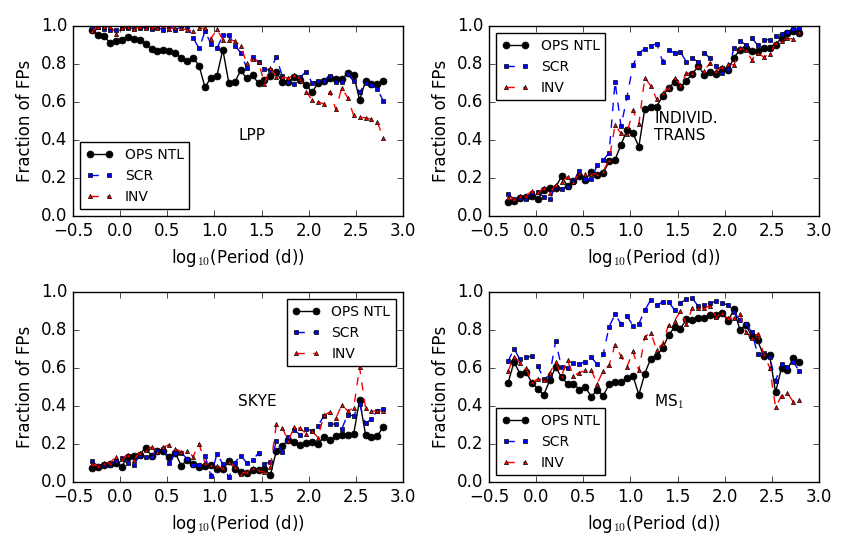
\includegraphics[width=0.9\linewidth]{fig-fractionFailsByMetric.png}
    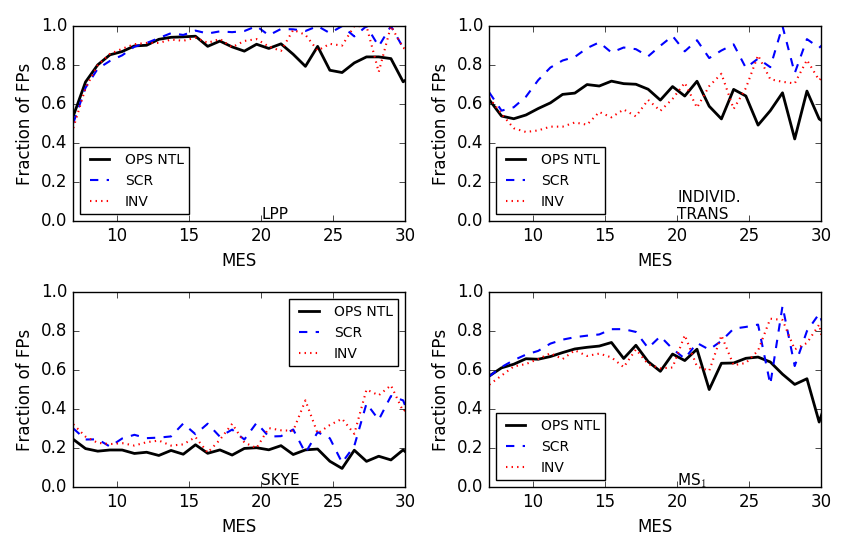
\includegraphics[width=0.9\linewidth]{fig-fractionFailsByMetricMes.png}
    \caption{The fraction of not-transit-like FPs failed by a particular Robovetter metric plotted against the logarithm of the period (top two rows) or linear MES (bottom two rows).  The fraction is plotted for the \opstce\ set in black, the \scrtce\ set in blue, and the \invtce\ set in red. The metric under consideration is listed on each plot.  For each metric we include fails from either detrending (DV or ALT). Upper left: LPP metric failures. Upper Right: TCEs that fail after removing a single transit due to any of the individual transit metrics.  Lower left: TCEs that fail after removing a single transit due to the Skye metric. Lower right: Model Shift 1 metric failures. Notice that there is a basic similarity between the trends seen in the three data sets, especially at long periods and low MES.}
    \label{f:fractionFailMetric}
\end{figure*}

%\begin{figure*}
%    \centering
    
%    \caption{The fraction of false positives failed by a particular type of Robovetter metric plotted against MES.  The fraction is plotted for not-transit-like FPs from the \opstce\ set in black, the \scrtce\ set in blue and the \invtce\ set in red. For each metric we include fails from either detrender (DV or Alt) for the metric stated in the middle of the plot. Upper left: LPP metric failures. Upper Right: TCEs that fails after removing a single transit due to any of the individual transit metrics.  Lower left: TCEs that fail after removing a single transit due to the Skye metric. Lower right: Model Shift 1 metric failures. }
%    \label{f:fractionFailMetricMes}
%\end{figure*}